\documentclass{beamer}

\usepackage{color}
\usepackage{graphicx}
\usepackage{amsmath}

\newcommand{\blue}[1]{\textcolor{blue}{#1}}
\newcommand{\red}[1]{\textcolor{red}{#1}}

\setbeamertemplate{frametitle}[default][center]

\begin{document}

\begin{frame}
\frametitle{DIII-D Discharge \#145380}

\begin{center}
\includegraphics[width=0.8\textwidth]{fig1.pdf}
\end{center}

\end{frame}

\begin{frame}
\frametitle{EPEC Simulation of DIII-D Discharge \#145380}

\begin{center}
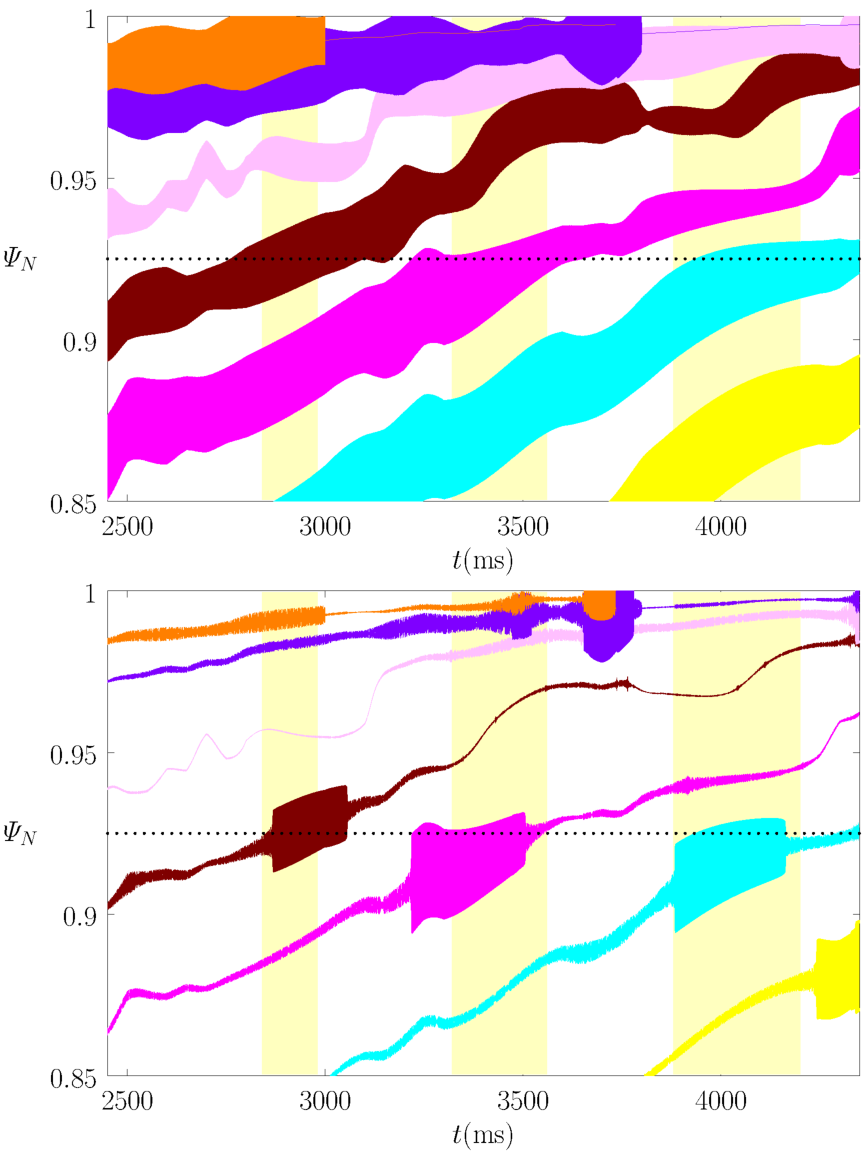
\includegraphics[width=0.6\textwidth]{fig9.pdf}
\end{center}

\end{frame}

\begin{frame}
\frametitle{Data Required by EPEC: 1) Plasma Equilibrium}

\begin{center}
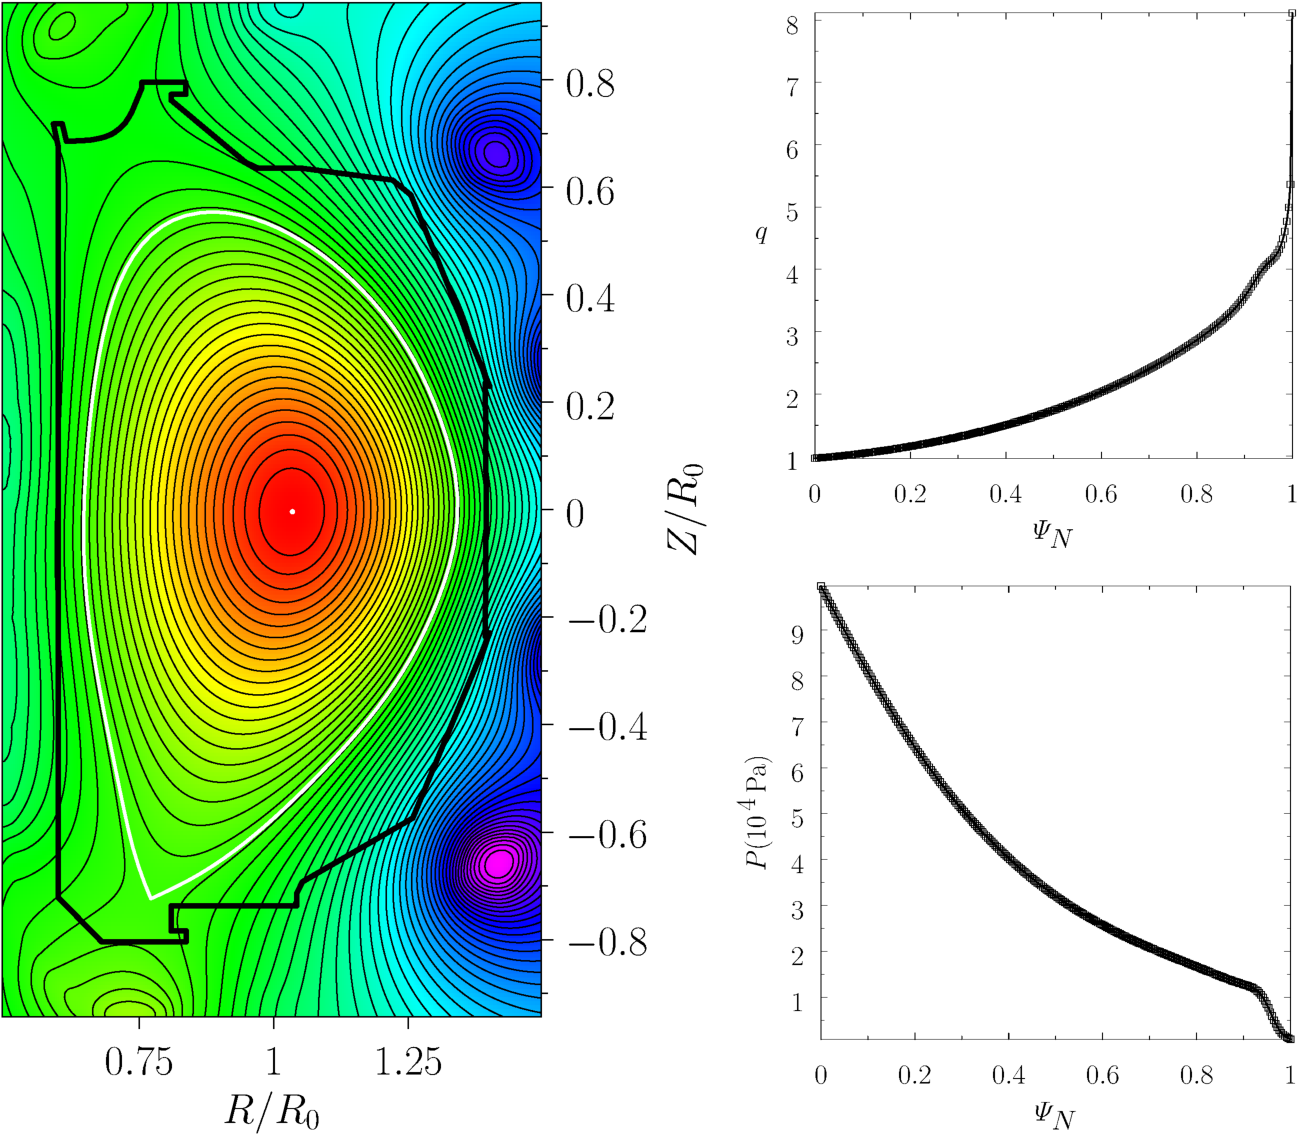
\includegraphics[width=0.8\textwidth]{fig2.pdf}
\end{center}

\end{frame}

\begin{frame}
\frametitle{Data Required by EPEC: 2) Plasma Profiles}

\begin{center}
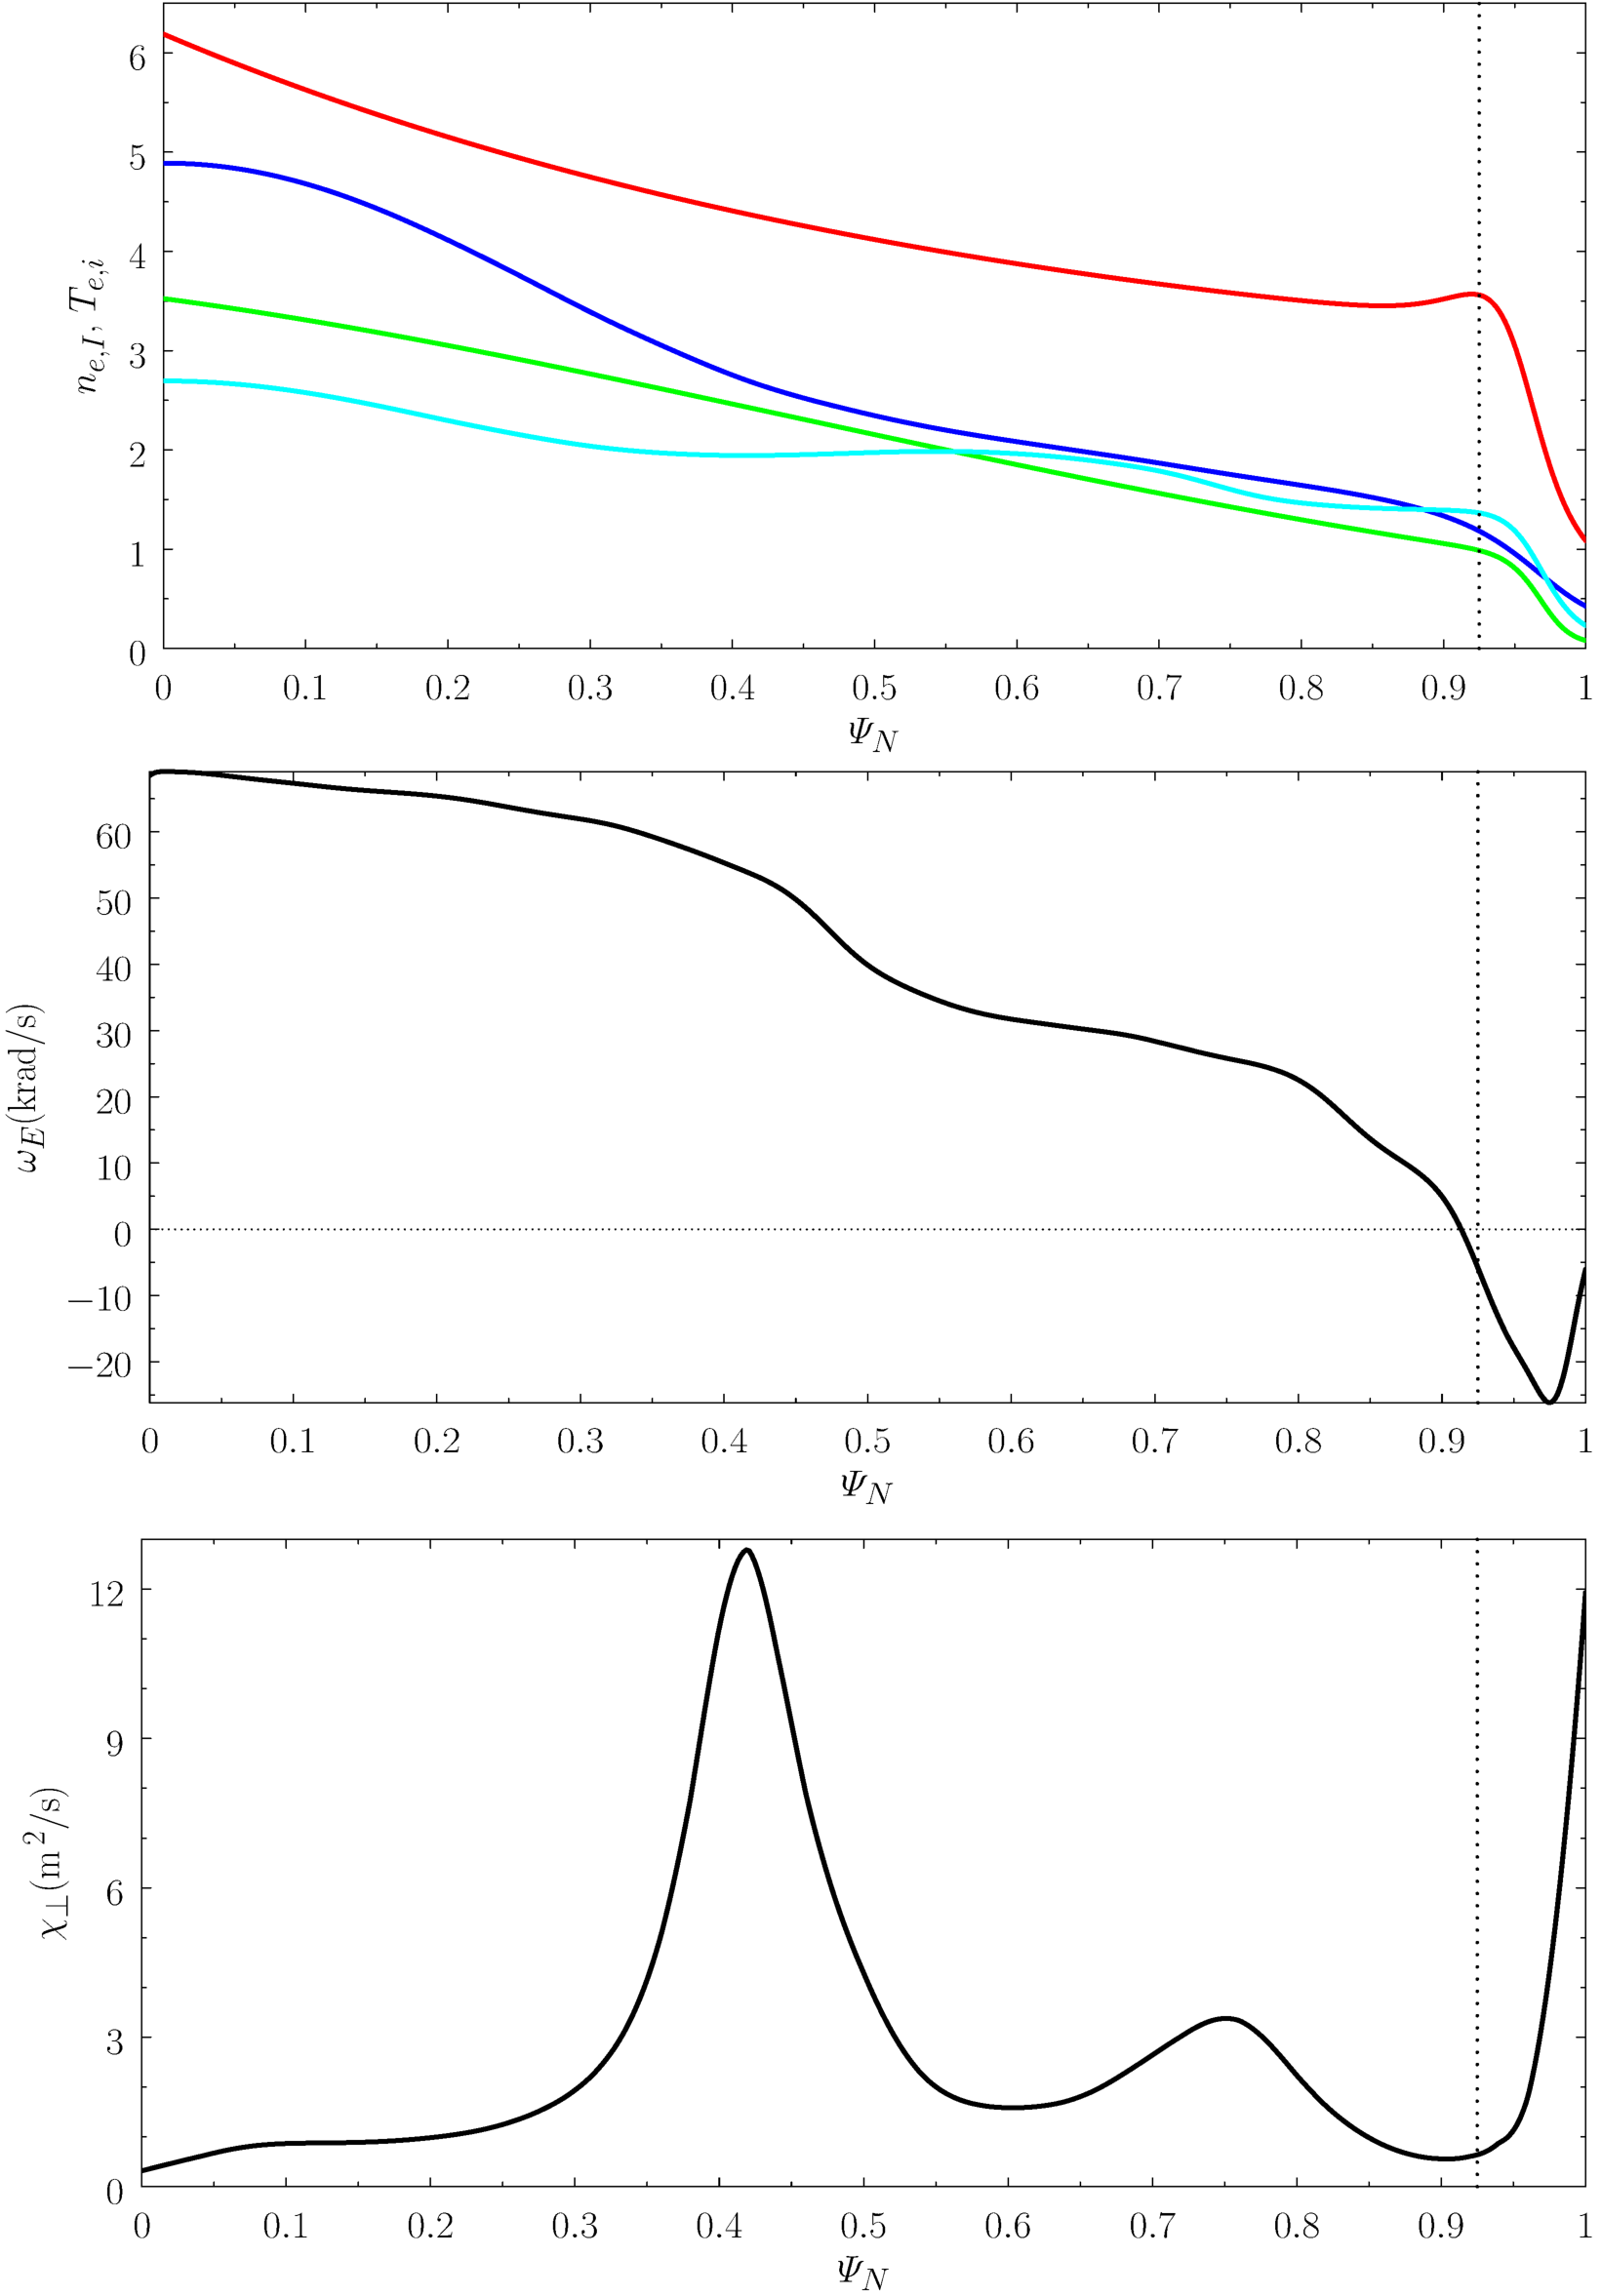
\includegraphics[width=0.5\textwidth]{fig3.pdf}
\end{center}

\end{frame}


\end{document}
